
%(BEGIN_QUESTION)
% Copyright 2014, Tony R. Kuphaldt, released under the Creative Commons Attribution License (v 1.0)
% This means you may do almost anything with this work of mine, so long as you give me proper credit

Solve for all voltages and currents in this series LR circuit:

$$\includegraphics[width=15.5cm]{i01034x01.eps}$$

Also, calculate the phase shift between $V_R$ and $V_{supply}$, as well as the phase shift between $V_L$ and $V_{supply}$.

\vfil

\underbar{file i01034}
\eject
%(END_QUESTION)





%(BEGIN_ANSWER)

This is a graded question -- no answers or hints given!

%(END_ANSWER)





%(BEGIN_NOTES)

{\bf Step 1:} Calculate all reactances ($X$).

\vskip 5pt

{\bf Step 2:} Draw an impedance triangle ($Z$ ; $R$ ; $X$), solving for $Z$

\vskip 5pt

{\bf Step 3:} Calculate circuit current using Ohm's Law: $I = {V \over Z}$

\vskip 5pt

{\bf Step 4:} Calculate series voltage drops using Ohm's Law: $V = {I Z}$

\vskip 5pt

{\bf Step 5:} Check work by drawing a voltage triangle ($V_{supply}$ ; $V_R$ ; $V_L$), solving for $V_{supply}$ using the Pythagorean Theorem

\vskip 5pt

{\bf Step 6:} Calculate the angle separating the $V_{supply}$ and $V_{R}$ sides of the voltage triangle by either taking the arc-cosine of $V_R \over V_{supply}$, or by taking the arc-sine of $V_L \over V_{supply}$, or by taking the arc-tangent of $V_L \over V_R$

\vskip 5pt

{\bf Step 7:} Calculate the angle separating the $V_{supply}$ and $V_{L}$ sides of the voltage triangle by either taking the arc-cosine of $V_L \over V_{supply}$, or by taking the arc-sine of $V_R \over V_{supply}$, or by taking the arc-tangent of $V_R \over V_L$

\vskip 5pt

{\bf Step 8:} Check work in steps 6 and 7 by ensuring that those two phase shift angles add up to 90$^{o}$

\vskip 10pt

$V_L = 12.60 \hbox{ volts RMS}$

\vskip 10pt

$V_R = 8.137 \hbox{ volts RMS}$

\vskip 10pt

$I = 11.46 \hbox{ milliamps RMS}$

\vskip 10pt

Phase shift between $V_R$ and $V_{source}$ = 57.15$^{o}$

\vskip 10pt

Phase shift between $V_R$ and $V_{source}$ = 32.85$^{o}$

%INDEX% Electronics review: AC reactance and impedance

%(END_NOTES)


